\newpage
\section{Virtualisation embarquée}
\subsection{Test de l'environnement EmbeddedXEN}
Tous les fichiers relatifs à l'environnement de virtualisation EmbeddedXEN, à l'exception du système
de fichiers (rootfs) préparé précédemment, se trouvent dans le répertoire embeddedxen situé dans votre
workspace.\\\\
\textbf{a) Donnée: }Le paramètre ex peut être utilisé avec le script deploy pour le déploiement des fichiers dans le rootfs
utilisé avec EmbeddedXEN, comme suit :
\begin{lstlisting}
$ ./deploy ex
\end{lstlisting}
Déployez les fichiers dans le nouveau \textit{rootfs}\\\\
\textbf{Travail réalisé: }Cette commande déploie les fichiers dans le rootfs de l'environnement de virtualisation.
\begin{lstlisting}
$ cd ~/seee_student/
$ ./deploy ex
Deploying into EmbeddedXEN rootfs ...
Mounting filesystem/reptar4-sdcard.img...
[sudo] password for redsuser: 
SD card partitions mounted in 'boot_tmp' and 'filesystem_tmp' directories
Unmounting SD card image...
Synchronizing .img file
Unmounting 'boot_tmp' and 'filesystem_tmp'...
Done !
$ 
\end{lstlisting}
\textbf{Remarque: }Il est très important de ne pas avoir de message d'erreur lors de l'exécution de cette commande. Si un message comme ci-dessous est observé, cela indique que l'image contenant le rootfs est corrompue. L'unique solution pour résoudre ce problème est de la télécharger à nouveau.
\begin{lstlisting}
mount: wrong fs type, bad option, bad superblock on /dev/loop1,
missing codepage or helper program, or other error
In some cases useful info is found in syslog - try
dmesg | tail  or so
\end{lstlisting}
\textbf{b) Donnée: }Démarrez le système en lançant le script ./stex.\\\\
\textbf{Travail réalisé: }Avec ce script on arrive dans l'U-boot et l'environnement graphique de la carte Reptar est lancé.
\begin{lstlisting}
$ ./stex
...
Reptar # 
\end{lstlisting}
\textbf{c) Donnée: }Vous pouvez observer le démarrage de l'hyperviseur, suivi du premier OS invité (Dom0), puis du
second OS invité (DomU). Les messages seront "mélangés" par la suite car les deux OS accèderont
simultanément à l'UART de la console. La commutation de la console entre Dom0 et DomU, puis
entre DomU et la console de l'hyperviseur, puis entre cette dernière et Dom0 de nouveau, s'effectue
à l'aide de trois combinaisons Ctrl-A successives (3 x Ctrl-A). Connectez-vous dans les deux
domaines (login et mot de passe : root).\\\\
\textbf{Travail réalisé: }Pour que l'hyperviseur démarre, il faut commencer par booter. On voit ensuite le démarrage de DOM-U, DOM-0 et l'hyperviseur XEN. À la fin du boot, on arrive dans le DOM-U où il faut entrer un mot de passe. Avec un Ctrl-A, on peut commuter la console et passer dans DOM-0. La capture ci-dessous présente les tests effectués. 
\begin{lstlisting}
Reptar # boot
...
*** Welcome on REPTAR (HEIG-VD/REDS): use root/root to log in ***
reptar login: [DOM-U] EXT2-fs (xvda1): warning: mounting unchecked fs, running e2fsck is recommended
[DOM-U] VFS: Mounted root (ext2 filesystem) on device 202:1.
[DOM-U] Freeing init memory: 88K
[DOM-U] ### HELLO FROM domU !!
...

[DOM-U] *** Welcome on REPTAR (HEIG-VD/REDS): use root/root to log in ***
reptar login: root
Password: 
# ls
Settings  config    qtrun

# *** Serial input -> DOMU (type 'CTRL-a' three times to switch input to Xen).
[DOM-0] <4>*** Serial input -> Xen (type 'CTRL-a' three times to switch input to DOM0).
[DOM-0] <4>*** Serial input -> DOM0 (type 'CTRL-a' three times to switch input to DOMU).
# ls
Settings  config    qtrun

# [DOM-0] <4>*** Serial input -> DOMU (type 'CTRL-a' three times to switch input to Xen).
[DOM-U] 
[DOM-U] *** Welcome on REPTAR (HEIG-VD/REDS): use root/root to log in ***
reptar login: 
\end{lstlisting}
\subsection{Déploiement du driver sp6 dans Dom0}
Dans cette étape, vous allez déployer votre driver sp6 dans Dom0. Pour cela, il faut d'abord le
recompiler pour le noyau correspondant à ce domaine.\\\\
\textbf{a) Donnée: }Modifiez le Makefile dans le répertoire drivers afin que la compilation du module s'effectue avec
le noyau linux-3.0-reptar-dom0 présent dans embeddedxen, et non plus avec le noyau linux-3.0-
reptar\\\\
\textbf{Travail réalisé: }La ligne suivante a été changée dans le Makefile pour compiler avec le noyau dom0.
\begin{lstlisting}
#KDIR	= ../linux-3.0-reptar
KDIR	= ../embeddedxen/linux-3.0-reptar-dom0
\end{lstlisting}
\textbf{b) Donnée: }Compilez votre module.\\\\
\textbf{Travail réalisé: }
\begin{lstlisting}
$ cd ~/seee_student/drivers/
$ make clean all
$ make
make -C ../embeddedxen/linux-3.0-reptar-dom0 
...
CC      /home/redsuser/seee_student/drivers/sp6.mod.o
LD [M]  /home/redsuser/seee_student/drivers/sp6.ko
make[1]: Leaving directory `/home/redsuser/seee_student/embeddedxen/linux-3.0-reptar-dom0'
$ 
\end{lstlisting}
\textbf{c) Donnée: }Déployez votre module dans le rootfs de Dom0 avec ./deploy ex .\\\\
\textbf{Travail réalisé: }
\begin{lstlisting}
$ cd ~/seee_student/
$ ./deploy ex
Deploying into EmbeddedXEN rootfs ...
Mounting filesystem/reptar4-sdcard.img...
[sudo] password for redsuser: 
SD card partitions mounted in 'boot_tmp' and 'filesystem_tmp' directories
Unmounting SD card image...
Synchronizing .img file
Unmounting 'boot_tmp' and 'filesystem_tmp'...
Done !
$
\end{lstlisting}
\textbf{d) Donnée: }Démarrez QEMU\\\\
\textbf{Travail réalisé: }
\begin{lstlisting}
$ cd ~/seee_student/
$ ./stex
...
Reptar # boot
...
\end{lstlisting}
\textbf{e) Donnée: }Dans Dom0, restez dans le répertoire /root, chargez le module puis lancez l'application ./qtrun :
\begin{lstlisting}
# cd
# insmod /sp6.ko
# ./qtrun
\end{lstlisting}
\textbf{Travail réalisé: }On voit ci-dessous que le driver est correctement inséré. lorsque l'on lance qtrun, cela va ouvrir QTextEdit dans la fenête Qemu que nous n'avions pas utilisée jusqu'ici. Cette fenêtre est une représentation graphique de l'écran tactile de la carte Reptar.
\begin{lstlisting}
# *** Serial input -> DOMU (type 'CTRL-a' three times to switch input to Xen).
[DOM-0] <4>*** Serial input -> Xen (type 'CTRL-a' three times to switch input to DOM0).
[DOM-0] <4>*** Serial input -> DOM0 (type 'CTRL-a' three times to switch input to DOMU).
# cd
# insmod /sp6.ko 
[DOM-0] <4>reptar_sp6: module starting...
[DOM-0] <4>Probing FPGA driver (device: fpga)
[DOM-0] <7>Registered led device: sp6_led0
[DOM-0] <7>Registered led device: sp6_led1
[DOM-0] <7>Registered led device: sp6_led2
[DOM-0] <7>Registered led device: sp6_led3
[DOM-0] <7>Registered led device: sp6_led4
[DOM-0] <7>Registered led device: sp6_led5
[DOM-0] <4>btns_reg address : 0xc5c18012
[DOM-0] <4>irq_reg address : 0xc5c1a018
sp6_read: Button irq status read 0x0 (button value 0x1)
sp6_write: Button irq status write 0x80
Enable IRQ
[DOM-0] <6>input: reptar_sp6_buttons as /devices/platform/fpga/reptar_sp6_buttons/input/input1
[DOM-0] <4>reptar_sp6: done.
# ./qtrun
\end{lstlisting}
Voici ci-dessous le contenu du script qtrun. On voit qu'il exécute les mêmes commandes que lorsque l'on a testé le driver des boutons dans le précédent labo. Les entrées sont liées au fichier /dev/input/event1.
\begin{lstlisting}
cd /usr/share/qt/demos/textedit
export QWS_KEYBOARD="LinuxInput:/dev/input/event1"
./textedit -qws
\end{lstlisting}
On peut tester que notre driver contrôlant les boutons fonctionne correctement en regardant la fenêtre QTextEdit. Lorsque l'on presse les boutons, on arrive a faire des espaces dans le texte, déplacer le curseur, mettre en gras...etc. On a donc un driver qui fonctionne dans Dom0 et ayant accès au matériel émulé.
\begin{figure}[H]
	\begin{center}
		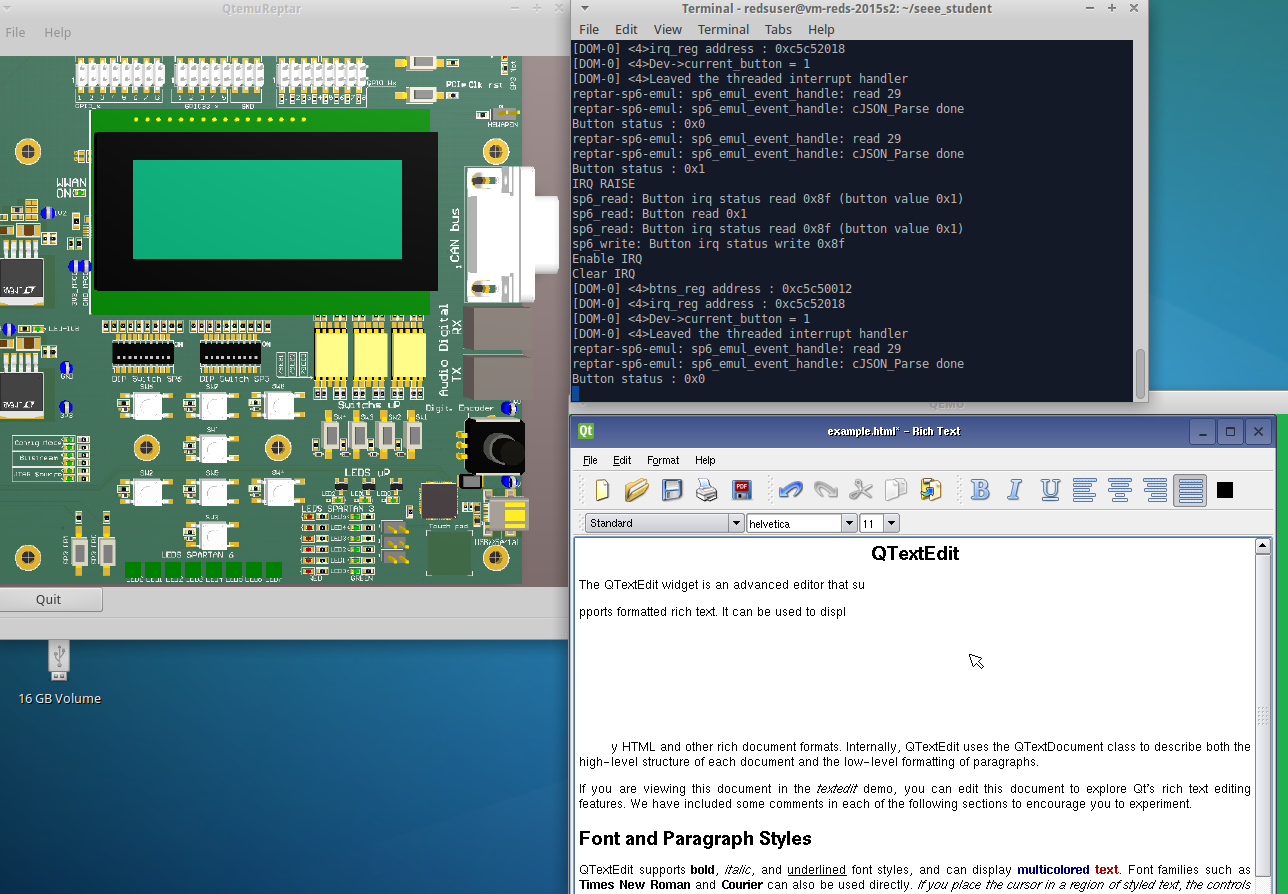
\includegraphics[width=16cm]{img/dom0.png}
		\caption{Exécution de Qtrun}
		\label{qtrun}
	\end{center}
\end{figure}
\subsection{Interaction entre Dom0 et DomU sur l'interface input para-virtualisé}
Dom0 peut accéder directement aux périphériques et les piloter, mais DomU ne le peut pas. Ainsi, nous
avons besoin de créer une interface virtuelle dans DomU pour lui permettre d’accéder aux ressources
du périphérique souhaité, en assurant une bonne coordination des accès. Les drivers sont découpés en
deux parties : le backend dans Dom0 et le frontend dans DomU.\\\\
Lors de cet exercice, nous allons permettre à l’application Qt dans DomU de récupérer les événements
input (input events) provenant de la FPGA.\\\\
\textbf{a) Donnée: }Identifiez les différents blocs qui interviennent lors de la propagation de l’input event depuis la
FPGA vers DomU. Etablissez un schéma faisant intervenir différents blocs : le backend input, le
driver FPGA développé par vos soins, le frontend input, les input subsystems de Dom0 et DomU…
(Vous trouverez le backend dans linux-3.0-reptar-dom0/drivers/input/xen-kbdback et le frontend
dans linux-3.4.6-domU/drivers/input/misc/xen-kbdfront.c ).\\\\
\textbf{Travail réalisé: }\\\\
\textbf{b) Donnée: }Modifiez votre driver afin que celui-ci s'enregistre auprès du backend input à l'aide de la fonction
xenvkbd\_inputdev\_register( ) (quelques indications sont fournies ci-après).\\\\
\textbf{Travail réalisé: }\\\\